\documentclass[12pt, a4paper]{report}

\usepackage{multicol}

% --- Packages de base ---
\usepackage[utf8]{inputenc}
\usepackage[T1]{fontenc}
\usepackage[french]{babel}
\usepackage{geometry}
\geometry{margin=2.5cm}

% --- Graphiques et Couleurs ---
\usepackage{graphicx}
\usepackage{xcolor}
\definecolor{primary}{RGB}{31, 73, 125} % Bleu scientifique
\usepackage[hidelinks]{hyperref} % Liens cliquables
\usepackage{pgfplots}
\pgfplotsset{compat=1.18}

% --- Mathématiques et Tableaux ---
\usepackage{amsmath, amssymb, amsthm}
\usepackage{booktabs} % Pour des tableaux professionnels
\usepackage{caption}
\usepackage[utf8]{inputenc}
\usepackage{multirow}
\usepackage[table]{xcolor} % Pour la couleur jaune des en-têtes

% --- Gestion du code (si besoin) ---
\usepackage{listings}
\lstset{basicstyle=\ttfamily\small, frame=single, breaklines=true}

% --- Page de Garde Personnalisée ---
\makeatletter
\def\subtitle#1{\gdef\@subtitle{#1}}
\def\institution#1{\gdef\@institution{#1}}
\def\logo#1{\gdef\@logo{#1}}


% --- faire de jolie source ---
\usepackage[most]{tcolorbox}


% --- logo de l'école ---
\usepackage{fancyhdr}
\pagestyle{fancy}
\setlength{\unitlength}{1mm}
\addtolength{\headheight}{1.5\baselineskip}
\renewcommand{\headrulewidth}{0.4pt}
\renewcommand{\footrulewidth}{0.4pt}
\rhead{
	
\includegraphics[width=2cm]{logo.png}
}

\renewcommand{\maketitle}{
	\begin{titlepage}
		\centering
		{\large \scshape \@institution} \par \vspace{1cm}
		\ifx\@logo\undefined \else \includegraphics[width=4cm]{\@logo} \fi \par \vspace{1.5cm}
		\rule{\linewidth}{0.5mm} \\[0.4cm]
		{\huge \bfseries \color{primary} \@title} \\[0.2cm]
		{\large \@subtitle} \\[0.4cm]
		\rule{\linewidth}{0.5mm} \\[1.5cm]
		
		\begin{minipage}{0.45\textwidth}
			\begin{flushleft} \large
				\emph{Auteur :}\\
				\@author \\
				Nicolas Hénin \\
				Roman Dufour
			\end{flushleft}
		\end{minipage}
		\begin{minipage}{0.45\textwidth}
			\begin{flushright} \large
				\emph{Encadrants :}\\
				Muriel Amiel \\
				Daniel Mazzoni
			\end{flushright}
		\end{minipage}
		
		\vfill
		{\large \@date}
	\end{titlepage}
}
\makeatother

% --- Informations du document ---
\institution{Centrale Méditerranée}
\logo{logo.png}
\title{Anémométrie par Température Constante}
\subtitle{Déterminer un profil de vitesse, qualifier la turbulance, et mettre en place un TP pour ECM}
\author{Nicolas Gallard}
\date{\today}


% --- DÉBUT DU DOCUMENT ---
\begin{document}
	
	\maketitle
	
	\tableofcontents
	
	\newpage
	
	\chapter{Introduction}
	L'anémométrie à fil chaud est une technique expérimentale de mesure des vitesses d'écoulement utilisée pour caractériser les fluctuations de vitesse dans des régimes turbulents. Basée sur la mesure de la dissipation thermique d'un fil métallique chauffé (en platine ou tungstène), cette méthode permet d'obtenir des mesures fines et rapides des composantes de vitesse locales dans un fluide, qu'il soit gazeux ou liquide. Ce système est très utilisé en dans la recherche et dans l'industrie, puisque les principes d'anémométrie sont directement liés à des problématiques de contrôle des écoulements en aéronautique, automobile ou thermique industrielle. \\
	
	L'objectif général est de maîtriser le fonctionnement du système d'anémométrie à fil chaud Dantec Streamline, installé dans la salle S07 du plot 6, et de proposer une étude expérimentale d'un jet turbulent dans un tube. \\
	
	
	L'enjeu de ce projet est double :
	
	\begin{itemizeFB}
	\item ● Scientifique : il s'agit de comprendre et d'expliciter les mécanismes physiques permettant l'utilisation de ce dispositif, tout en utilisant des outils numériques (Streamline, Comsol Multiphysics) pour modéliser le phénomène ;
	\item ● Pédagogique: puisqu'il vise à concevoir un TP, et un support expérimental pour la mesure de vitesse.
	\end{itemizeFB}
	
	Nous utiliserons le principe d'\textbf{Anémométrie par Température Constante} pour le projet, car nous n'avons pas l'équipement nécessaire pour faire les mesures en \textbf{Anémométrie par Courant Constant}, Voici un comparatif rapide entre les deux méthodes:
	
	\begin{table}[h!]	
		\centering
		\label{tab:ACC & ATC}
		\resizebox{\textwidth}{!}{
			\begin{tabular}{lcc}
				\toprule
				& \cellcolor{red!20}\textbf{ACC (Courant Constant)} & \cellcolor{green!20}\textbf{ATC (Température Constante)} \\
				\midrule
				\textbf{Principe} & Intensité $I$ maintenue fixe & Résistance $R$ (et Température) fixe \\
				\textbf{Variable mesurée} & Variations de tension $V$ & Courant d'asservissement \\
				\textbf{Temps de réponse} & Lent (Inertie thermique du fil) & Très rapide (Boucle d'asservissement) \\
				\textbf{Compensation} & Requiert un circuit externe lourd & Automatique par le pont de Wheatstone \\
				\textbf{Étude turbulence} & Limitée aux basses fréquences & Jusqu'à plusieurs centaines de kHz \\
				\midrule
				\textbf{Statut} & \textbf{Obsolète} & \textbf{Retenue} \\
				\bottomrule
			\end{tabular}
		}
		\caption{Comparaison des méthodes d'anémométrie à fil chaud}
	\end{table}

	
	\chapter{Matériel et Méthodes}
	
	\section{Protocoles possibles}
	Un premier protocole de calibration dit "élémentaire", pour faire fonctionner et relever des valeurs par la sonde pourra être le premier à mettre en place: Relever une vitesse pour mesure un nombre de Reynold et qualifier la turbulence, et confronter la méthode à une autre comme peut permettre les tubes de Pitot.\\
	
	
	Avec le matériel à disposition dans le local de TP, nous pourrions selon la bibliographie faire ces protocoles plus complets:

	\begin{tcolorbox}[colback=gray!5, colframe=gray!50, arc=0mm, title=Suggestions de Protocoles expérimentals par Dantec Dynamics]
		\tiny
		\textbf{1/ Très basses vitesses}\\
		À de très basses vitesses, le transfert de chaleur du fil est régi par la convection naturelle. Cela signifie que le refroidissement ne dépend pas seulement de l'amplitude de la vitesse, mais aussi de son orientation par rapport au champ de gravité. L'influence de la convection naturelle commence autour de 0,2 m/s pour les sondes à fil et prend totalement le dessus aux alentours de 0,03-0,04 m/s. Dans cette plage, il est important que la sonde garde la même orientation par rapport au champ de vitesse lors de l'étalonnage et de la mesure.\\
		
		\textbf{2/ Hautes vitesses et écoulements compressibles}\\
		À des vitesses élevées, l'écoulement devient compressible et les effets de compressibilité doivent être pris en compte. En pratique, cela signifie que la pression et la vitesse doivent être mesurées simultanément. La correction est assez complexe et est très souvent négligée.\\
				
		\textbf{3/ Effets de paroi}\\
		Lorsque le fil est placé à proximité d'une paroi solide, la chaleur est conduite à travers le fluide vers la paroi. Si cela n'est pas corrigé, la vitesse mesurée sera surestimée. L'influence de la paroi commence à une distance adimensionnelle $y^+ = y U_{\tau} / \nu = 3,5$ (où $y$ est la distance à la paroi, $U_{\tau}$ la vitesse de frottement et $\nu$ la viscosité cinématique). La distance critique à la paroi est typiquement de 0,1 à 0,2 mm, selon la vitesse de l'écoulement libre.\\
		
		\textbf{4/ Très haute turbulence et écoulements avec inversible}\\
		Si la turbulence est très élevée (au-dessus de 30\% ou plus) ou dans des écoulements avec inversion de sens, où le vecteur vitesse sort de l'angle d'ouverture du réseau de capteurs, les résultats seront incorrects. De tels écoulements peuvent être mesurés correctement avec des systèmes de fil chaud volant (flying hot-wire), où la sonde est déplacée à travers le champ d'écoulement à une vitesse suffisamment élevée pour maintenir le vecteur vitesse résultant à l'intérieur de l'angle d'ouverture. Après linéarisation, la vitesse de déplacement de la sonde est soustraite de la composante longitudinale de la vitesse."
		
		\tcblower
		\footnotesize \textbf{Source :} \url{Bibliographie}
	\end{tcolorbox}
	
	Il existe une variété importante de sonde d'anémomètrie, pour faire d'autres études avec ces sondes. On pourra citer l'exemple de la très faible vitesse, où une boule chaude sera plus adaptée à la situation.
	
	\section{Dispositif expérimental}
	En suivant les suggestion de Dantec Dynamics, nous partirons pour une mesure à haute vitesse, mais nous considérons un écoulement incompressible, et qui ne s'inverse pas.\\
		
	Nous avons ici un dispositif expérimental utilisant l'effet Joule, nous devrons donc faire appel à la théorie de la thermodynamique, et électique. Commençons par un bilan thermique sur le fil chaud, on retiendra \textbf{quatres transferts thermiques} dans le bilan thermique du fil chaud:
	
	\begin{itemize}
		\item Conduction vers le fluide, due à la diffusion moléculaire de la chaleur dans le fluide;
		\item Convection vers le fluide, où la chaleur est transportée par le mouvement du fluide	environnant;
		\item Conduction vers les supports, due à la diffusion de la chaleur le long du fil;
		\item Rayonnement thermique : puissance transférée sous forme de rayonnement électromagnétique.
	\end{itemize}

	Par rapport aux quatre échanges thermiques dans ce système, on pourra négliger dans cette étude les deux transferts suivants:
	\begin{itemize}
		\item Conduction vers les supports;
		\item Rayonnement thermique.
	\end{itemize}
	
	On négligera le rayonnement thermique qui est minime par rapport aux deux premiers transferts. Et grâce au fait que $d << l$ (facteur 100) dans le fil chaud, alors on pourra négliger la conduction vers les supports. \\
	
	Par permier \textbf{principe de la thermodynamique} sur le système fil chaud
	\begin{center}
		$\partial_t U = \Sigma P = P - \dot{Q} $
	\end{center}
	Avec les expressions suivantes pour $P$ la puissance émise par effet Joule, et $\dot{Q}$ l'échange temporelle avec le milieu extérieur:
	\begin{itemize}
		\item $\dot{Q} =  h S (T_w - T_0)$
		\item $P = R_{w} I^2$
	\end{itemize}
	
	Avec les constantes suivantes définies :
	\begin{itemize}
		\item $h$ le coefficient de dissipation avec l'extérieur;
		\item $S$ surface latérale du fil chaud;
		\item $T_w$ température du fil chaud;
		\item $T_0$ température du milieu extérieur;
		\item $R_w$ résistance du système "fil d'anémométrie";
		\item $I$ Intensité électrique dans le fil chaud.
	\end{itemize}
	
	
	On supposera pour que $T_w$ est identique sur toute la longueur du fil, et nous travaillerons avec le nombre adimensionné de Nusselt, et développant S = "surface latérale du fil chaud" = $d*\pi$, avec d le diamètre du fil chaud : \\
	\begin{center}
		$\mathrm{Nu} = \frac{h d}{k_f}$; \quad $\dot{Q} = \pi l k_f (T_w - T_0)\,\mathrm{Nu}$
	\end{center}
	
	Avec :
	\begin{itemizeFB}
		\item $k_f$ : coefficient de diffusion thermique.
	\end{itemizeFB}
	
	D'où la relation suivante :
	\begin{center}
		$\partial_t U = R_w I^2 - \pi l k_f (T_w - T_0)\,\mathrm{Nu}$
	\end{center}
	
	
	Nous obtenons le premier résultat pour le fil chaud, en prenant l'hypothèse que $\partial_t U = 0 $, soit le \textbf{régime stationnaire}. On obtient une première équation fondamentale pour l'expérience:
	\begin{center}
		\boxed{R_w I^2 = \pi l k_f (T_w - T_0)\,\mathrm{Nu}}
	\end{center}
	
	
	\section{Caractéristiques dynamiques et limite de fréquence}
	On pourra se poser la question suivante : "Combien de temps il serait nécessaire d'attendre pour stabiliser la valeur du nombre de Reynold?". Dans l'étude du fil chaud, un terme de stockage de chaleur est ajouté à l'équation de transfert thermique stationnaire pour rendre compte des variations temporelles :
	\begin{equation*}
		I^2 R_w = (R_w - R_0)(A + B U^n) + C_w \frac{dT_w}{dt}
	\end{equation*}
	
	En exprimant la température du fil $T_w$ en fonction de sa résistance $R_w$ et de son coefficient de température $\alpha_0$, on obtient l'équation différentielle suivante :
	\begin{equation*}
		I^2 R_w = (R_w - R_0)(A + B U^n) + \frac{C_w}{\alpha_0 R_0} \frac{dR_w}{dt}
	\end{equation*}
	
	
	\begin{figure}[h]
		\centering
		\begin{minipage}{0.48\linewidth}
			Cette équation définit une constante de temps $\tau$ :
			\begin{equation*}
				\tau = \frac{C_w}{\alpha_0 R_0 (A_1 + B_1 U^n - I^2)}
			\end{equation*}
		\end{minipage}
		\hfill
		\begin{minipage}{0.375\linewidth}
			\centering
			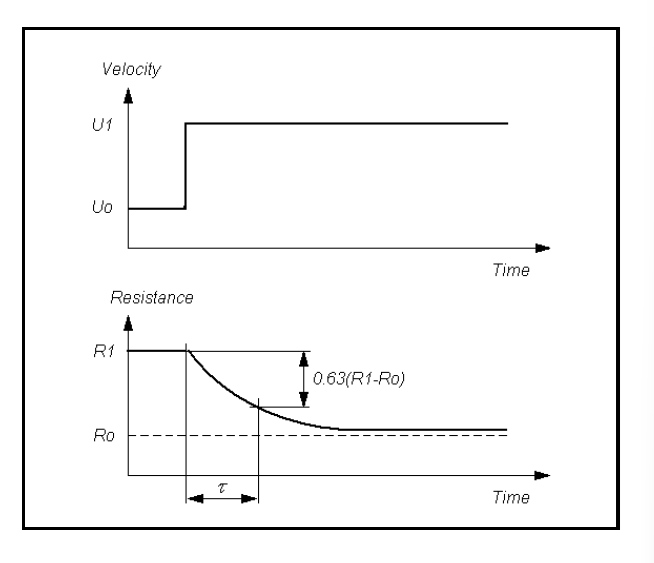
\includegraphics[width=\linewidth]{Images/0 graphique.png}
			\caption{Représentation graphique du pas temporelle $\tau$}
		\end{minipage}
	\end{figure}

	On pourra alors définir une fréquence limite donnée par :
	\begin{equation*}
		\boxed{f_{cp} = \frac{1}{2\pi\tau}}
	\end{equation*}
	Cette fréquence est une estimation pertinente pour deux situations. Elle représente la fréquence maximale où l'on peut relever des valeurs pour une variation brutale de la vitesse incidente. En fonction de la valeur de $\tau$ ou $f_{cp}$, on pourra répondre à ces deux questions:
	\begin{itemize}
		\item Combien de temps il faut attendre entre deux prises de mesure de vitesse ?
	Soit faire la mesure de $U_{21} = 3 m/s$, à $U_{22} = 3,5 m/s$;
		\item Jusqu'à quelle variation de vitesse spontanée, nous n'aurons plus de valeur stable ?
	Soit si le courant faire des va-et-vient (situation de turbulance forte), quelle est la limite de la fréquence de va-et-vient ?
	\end{itemize}
	
	
	
	
	\chapter{Dispositif expérimental}
	\section{Présentation du matériel mis à disposition}
	Voici les différents éléments composants le montage de l'expérience : \\
	% --- Groupe 1 : Montages sortie tuyau ---
	\begin{figure}[h]
		\centering
		\begin{minipage}{0.48\textwidth}
			\centering
			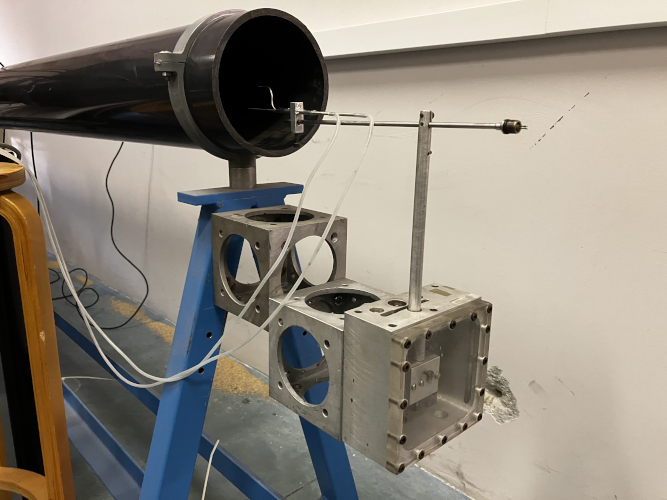
\includegraphics[width=\linewidth]{Images/1 montage sortie tuyau 1 small.png}
			\caption{Montage sortie tuyau (vue 1)}
		\end{minipage}
		\hfill
		\begin{minipage}{0.375\textwidth}
			\centering
			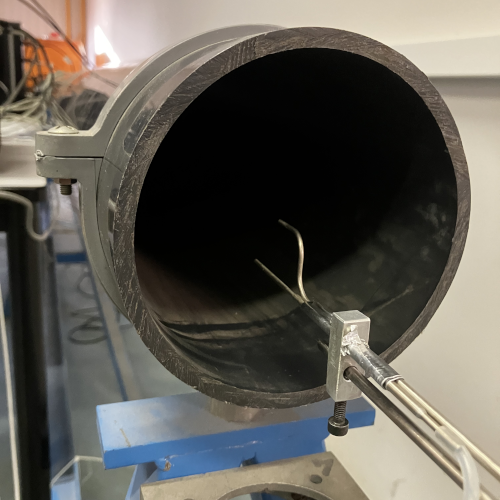
\includegraphics[width=\linewidth]{Images/2 montage sortie tuyau 2 small.png}
			\caption{Montage sortie tuyau (vue 2)}
		\end{minipage}
	\end{figure}
	
	
	Nous avons sur les figures 3.1, et 3.2 l'installation presque complètent à la sortie du cylindre. On y observera: \\
	\begin{itemize}
		\item le cylindre en PVC;
		\item le support métallique pour les capteurs;
		\item le système associé aux tubes de Pitot.
	\end{itemize}
	Sur la figure 3.2, on aura un zoom sur la sortie et la manière dont on a disposé les tubes de Pitot. On mesure la pression statique avec le tube droit, et la pression dynamique avec le tube coudé. \\
	
	Nous avons relevé des valeurs selon l'axe z dans le référentiel terrestre, ce qui nous a permis de faire des mesures selon  un axe radial du cylindre, en particulier , celui parallèle à l'axe z terrestre. Par la géométrie du système, la mesure sur un axe radial complet du cylindre, permet d'avoir le profil du vitesse sur sa tranche, par invariant de rotation du profil de vitesse.
	
	
	\newpage
	% --- Groupe 2 : Instrumentation et Acquisition ---
	\begin{figure}[h]
		\centering
		\begin{minipage}{0.31\textwidth}
			\centering
			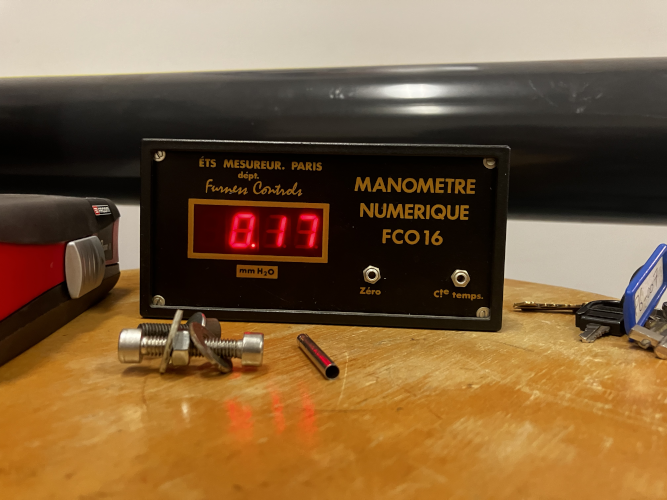
\includegraphics[width=\linewidth]{Images/3 Manometre small.png}
			\caption{Manomètre différentiel}
		\end{minipage}
		\hfill
		\begin{minipage}{0.31\textwidth}
			\centering
			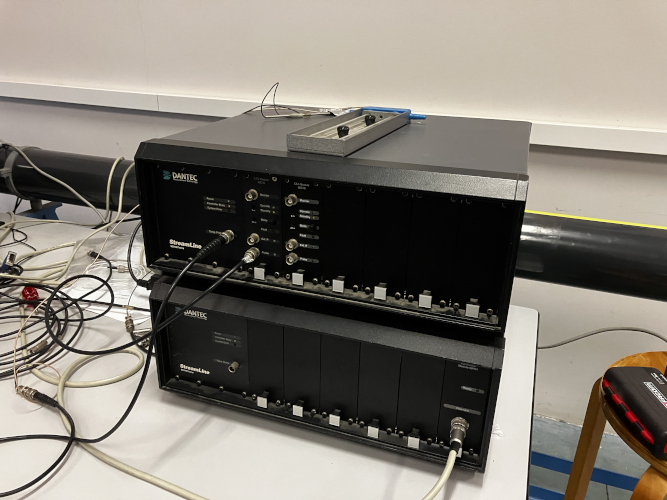
\includegraphics[width=\linewidth]{Images/4 Streamlines Hardware small.png}
			\caption{Matériel StreamLine}
		\end{minipage}
		\hfill
		\begin{minipage}{0.31\textwidth}
			\centering
			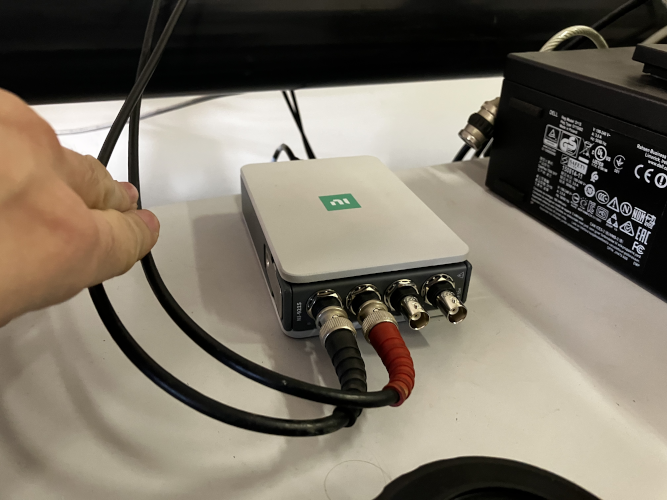
\includegraphics[width=\linewidth]{Images/5 Boitier acquisition small.png}
			\caption{Boîtier d'acquisition}
		\end{minipage}
	\end{figure}
	
	Les figures 3.3, 3.4, et 3.5 représentent les instruments de mesure hardware du système.
	\begin{itemize}
		\item 3.3 : manomètre utilisé pour la mesure de la pression statique dans le système. Il indique le différentiel de pression en $mmH_2O$ grâce à aux tubes de Pitot;
		\item 3.4 : Boitiers StreamLine permettant l'acquisition des valeurs de la sonde fil chaud
		\item 3.5 : Boitier IU permettant le formatage des données du boitier StreamLine au logiciel StreamWare dans l'ordinateur.
	\end{itemize}
	Ce sont les instruments minimums supplémentaires pour l'acquisition de données pour l'utilisation des tubes de Pitot (Manomètre), et le fil chaud (StreamLine, IU, et ordinateur). 
	
	
	% --- Groupe 3 : Sondes fil chaud ---
	\begin{figure}[h!]
		\centering
		\begin{minipage}{0.45\textwidth}
			\centering
			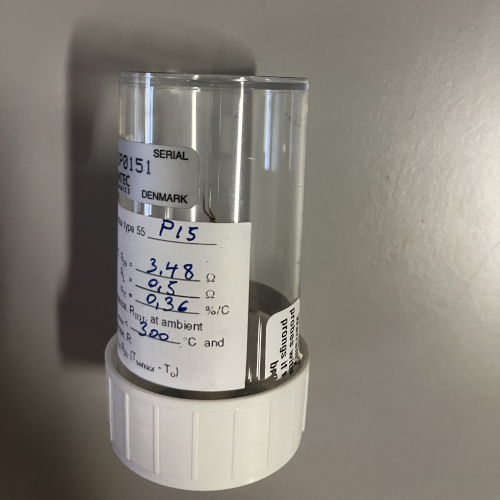
\includegraphics[width=0.75\linewidth]{Images/6 fil chaud 1 small.png}
			\caption{Sonde à fil chaud (verticale)}
		\end{minipage}
		\hfill
		\begin{minipage}{0.45\textwidth}
			\centering
			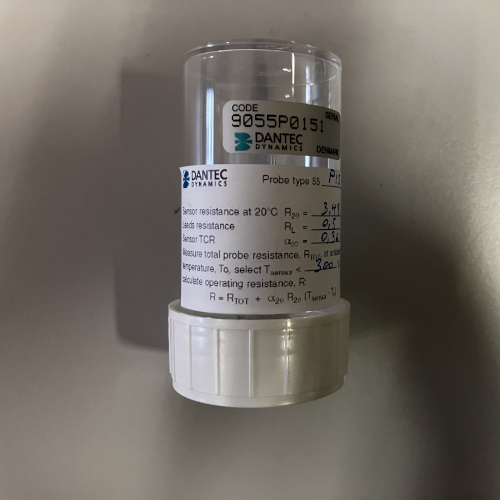
\includegraphics[width=0.75\linewidth]{Images/7 fil chaud 2 small.png}
			\caption{Détail de la sonde à fil chaud}
		\end{minipage}
	\end{figure}
	Voici un exemple de présentation d'un fil chaud, on peut y lire que l'étiquette que nous avons affaire à un fil chaud coudé 1D de référence $55P15$, avec les constantes suivantes:
	\begin{itemize}
		 \item \textbf{R\_20} : 3,48 $\Omega$; 
		 \item \textbf{R\_L} : 0,5$\Omega$;
		 \item \textbf{alpha\_20} : 0.36 $\%/°C$;
		 \item \textbf{T\_max} : 300 $°C$
	\end{itemize}
	Nous avons fait un \textbf{tableau récapitulatif} de toutes les sondes d'Anémométrie par Température Constante dans la page suivante, avec leurs constantes respectives.
	
	
	
	
	
	\section{Précaution nécessaire}
	L'arrangement du matériel dans la salle de TP n'a pas besoin d'être modifié. Il y aura seulement les tubes de Pitot, et le fil chaud avec son support qui seront déplacés pendant les manipulations.
	
	\textbf{Précaution à suivre} pour le bon déroulement du TP:
	\begin{itemizeFB}
		\item Un nettoyage du tube PVC sera nécessaire pour éviter que les poussières endommagent ou cassent les fils chaud;
		\item Le support étant de taille petite, les manipulations des supports, des tubes, ou du fil devront être minimisées;
		\item Le manomètre différentiel devra être le plus proche du support visible en figure 3.1, il faudra éviter de le mettre par terre, ou de le faire tomber.
	\end{itemizeFB}
	
	
	
	
	\section{Solution Dantec Dynamics}
	\subsection{Présentation de la solution}
		
	\begin{tcolorbox}[colback=gray!5, colframe=gray!50, arc=0mm, title=Description officielle]
		\tiny
		"Le domaine d'activité principal de DANTEC DYNAMICS est le développement et la vente de systèmes de mesures intégrés pour le diagnostic et la recherche en mécanique des fluides, mécanique des solides, microfluidique, analyse des sprays et technologie de la combustion.\\
		
		
		Nos systèmes sont utilisés pour obtenir des données de mesure des propriétés physiques dans l'air, dans des gaz, dans des liquides et dans des solides.\\
		
		
		Les paramètres étudiés sont par exemple la vitesse, la turbulence, la taille des particules, la concentration, la température, le type de combustion, les contraintes/déformations et les vibrations."
		
		\tcblower
		\footnotesize \textbf{Source :} \url{https://www.dantecdynamics.com/fcs/presentation-de-la-societe/}
	\end{tcolorbox}
	
	La présentation de la société sur son site internet montre que nous avons affaire à des outils de précision, permettant la mesure de constantes physiques parfois non triviale ou avec une précision remarquable. On pourra citer la qualification de la turbulence, qui n'est pas accessible à tous les outils de mesure sur le commerce.
	

	
	
	\subsection{Le hardware et StreamWare : les composants physiques}
	
	Nous avons plusieurs fils chauds à notre disposition, et on pourra prendre l'exemple du fil en Figure 3.6, de \textbf{référence 55P15} : il permet de relever une tension ou intensité électrique permettant la mesure d'une vitesse locale. Ici, nous avons un fil chaud 1D coudé, on pourra alors mesurer, avec le reste des composants de la solution Dantec Dynamics, une vitesse selon une unique composante de l'espace. Avec autant de points que la fréquence de l'ensemble le permet, soit des fréquences de l'ordre du $kHz$.\\
	
	Une section est dédiée à cette partie, car la solution prend en compte tous les composants du protocole pour permettre le relevé de la mesure.
	
	\begin{figure}[h]
		\centering
		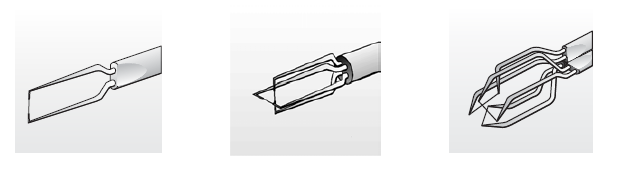
\includegraphics[width=0.50\linewidth]{Images/8 fil chaud xD.png}
		\caption{Figure 3.8, de gauche à droite, fil chaud 1D, 1D deux fils, et 3D}
	\end{figure}
	
	Sur la figure 3.8, nous pouvons voir comment on distingue les fils chauds 1D à 3D. Elles se différencient par le nombre de fil, mais aussi de leur placement. En effet, celui de droite est un fil chaud 3D, et permet la mesure de toutes les composantes de la vitesse dans l'espace, puisque chaque sonde permet une mesure de la composante de la vitesse selon une incidence arrivant sur la tranche du fil.
	
	\subsection{Le software StreamLine : Le logiciel}
	
	
	
	\begin{figure}[h!]
		\centering
		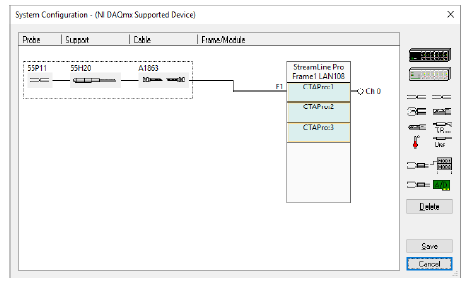
\includegraphics[width=0.90\linewidth]{Images/9.1 reglage streamline.png}
		\caption{Fenêtre d'initialisation, et dimensionnement du matériel}
	\end{figure}
	
	Sur la Figure 3.9, nous avons la \textbf{fenêtre type du logiciel Streamline avant l'acquisition des données}, soit décrire numérique le matériel du protocole mis en place. Nous devrons lire cette fenêtre comme un tableau contenant les pictogrammes des composants physiques. \\
	
	Par exemple, ici nous retrouvons dans la colonne "Probe", tout à gauche du tableau, le fil chaud, avec la référence "55P11", mais le logiciel prend en compte en plus le "Support" et le "Cable", qui sont respectivement le support, et le cable utilisés pour la manipulation. Il y a une pertinence physique, car nous avons affaire à un système électronique, donc toutes les résistances devraient être prisent en compte. En effet, on n'aura pas la même résistance sur le cable, s'il n'est pas de la même longueur, épaisseur, matière, ...\\
	\textbf{C'est sans doute la force de cet outil : le logiciel est simple mais complexe, au prix d'une inertie à sa maîtrise est importante.}
	
	\newpage
	\begin{figure}[h]
		\centering
		\begin{minipage}{0.45\textwidth}
			\centering
			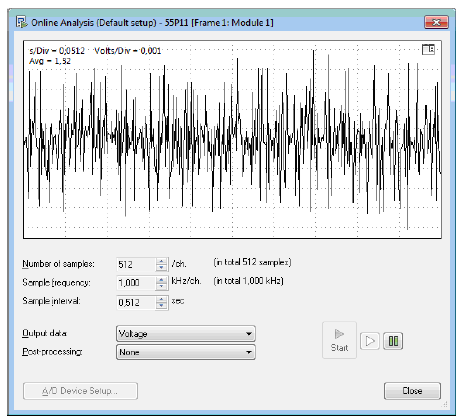
\includegraphics[width=0.80\linewidth]{Images/9.2 resultat graphique.png}
			\caption{Résultat brut de l'acquisition du fil chaud}
		\end{minipage}
		\hfill
		\begin{minipage}{0.45\textwidth}
			\centering
			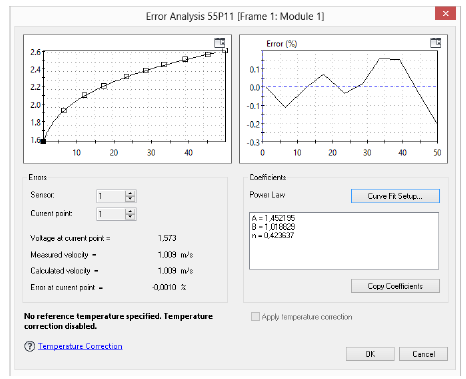
\includegraphics[width=0.90\linewidth]{Images/9.3 erreur graphique.png}
			\caption{Estimation de l'erreur}
		\end{minipage}
	\end{figure}
	
	Dans la Figure 3.10, nous avons les résultats brutes du système modélisé en Figure 3.9. L'abscisse du graphique représente l'échelle temporelle, et l'axe des ordonnées représente la tension. L'intérêt de la sonde est qu'elle permet de \textbf{quantifier deux éléments}: la valeur moyenne de la vitesse, et les variations instantanées de tension dans le tube.\\
		
	La Figure 3.11 est la deuxième fenêtre d'information que l'on obtient, soit \textbf{l'erreur sur les mesures de la sonde}. Elle nous fournie 3 éléments:
	\begin{itemize}
		\item 1 - (en haut à gauche) un tracé de l'erreur dimensionné;
		\item 2 - (en haut à droite) un tracé de l'erreur en pourcentage;
		\item 3 - les coefficients de corrélation associés à une loi de puissance.
	\end{itemize}
	
	
	\section{Lecture des graphiques sur l'exemple}
	\subsection{Présentation du matériel et configuration}
	Les mesures ont été effectuées à l'aide d'un système \textbf{Dantec Dynamics}. La configuration expérimentale repose sur une sonde fil chaud de type \textbf{55P11}, montée sur un support \textbf{55H20} et reliée par un câble \textbf{A1863} au module d'acquisition \textbf{CTA Pro} (châssis LAN108)\\
	
	
	L'acquisition a été paramétrée avec les réglages suivants :
	\begin{itemize}
		\item Nombre d'échantillons : 512
		\item Fréquence d'échantillonnage : 1,000 kHz
		\item Temps d'intégration : 0,512 s
	\end{itemize}
	
	\subsection{Modèle de conversion et étalonnage}
	La transition entre la tension mesurée $E$ et la vitesse du fluide $U$ suit une loi de puissance (Loi de King modifiée), définie par les coefficients extraits de l'étalonnage :
	\begin{equation}
		E^2 = A + B U^n
	\end{equation}
	
	D'après les résultats de la Figure 3.11, les coefficients, pour la corrélation avec une loi puissance, retenus sont :
	\begin{itemize}
		\item $A = 1,452195$;
		\item $B = 1,018829$;
		\item $n = 0,423637$.
	\end{itemize}
	
	\subsection{Valeurs mesurées et estimation de l'erreur}
	Pour un point de mesure stabilisé, nous obtenons les valeurs suivantes :
	\begin{itemize}
		\item \textbf{Tension mesurée :} $1,573$ V;
		\item \textbf{Vitesse calculée ($U$) :} $1,009$ m/s.
	\end{itemize}
	
	L'estimation de l'erreur systématique, calculée par la différence entre la vitesse mesurée et la courbe de tendance (Curve Fit), est extrêmement faible pour ce point :
	\begin{equation}
		\epsilon_{vitesse} = -0,0010 \%
	\end{equation}
	
	\subsection{Caractérisation de l'écoulement}
	À partir de la vitesse $U \approx 1,01$ m/s, nous pouvons calculer le nombre de Reynolds $Re$, avec $D$ le diamètre équivalent du conduit :
	\begin{equation}
		Re = \frac{U D}{\nu}
	\end{equation}
	Où $\nu$ est la viscosité cinématique de l'air ($\approx 1,5 \cdot 10^{-5}$ m$^2$/s à 20°C).
	
	
	
	
	\chapter{Résultats et Discussion}
	\section{Matériel Disponible}
	Présentation des graphiques et interprétation des phénomènes observés.
	
	\begin{table}[h!]
		\centering
		\label{tab:inventaire_fil_chaud}
		\resizebox{\textwidth}{!}{
			\begin{tabular}{lcccccc}
				\toprule
				\textbf{Référence} & \textbf{Type de fil} & \textbf{R\_20 } & \textbf{R\_L} & \textbf{alpha\_20 } & \textbf{T\_max } & \textbf{État} \\
				& & ($\Omega$) & ($\Omega$) & ($\%/°C$) & ($°C$) & \\
				\midrule
				Probe Type 55 R11 & 1D/droit & 3,3 & 0,5 & 0,48 & 150 & Non vérifié \\
				Probe Type 55 R11 & 1D/droit & 6 & 0,5 & 0,4 & 300 & Non vérifié \\
				Probe Type 55 R11 & 1D/droit & 6,2 & 0,5 & 0,37 & 150 & Non vérifié \\
				Probe Type 55 R11 & 1D/droit & 6,7 & 0,5 & 0,36 & 150 & Non vérifié \\
				Probe Type 55 R11 & 1D/droit & 7,07 & 0,6 & 0,4 & 150 & Non vérifié \\
				Probe Type 55 R11 & 1D/droit & 8,6 & 0,6 & 0,42 & 150 & Non vérifié \\
				Probe Type 55 R01 & 1D/droit & 5,3 & 0,5 & 0,48 & 300 & Non vérifié \\
				\midrule
				Probe Type 55 P15 & 1D/coudé & 3,3 & 0,5 & 0,36 & 300 & Non vérifié \\
				Probe Type 55 P15 & 1D/coudé & 3,4 & 0,5 & 0,36 & 300 & Non vérifié \\
				Probe Type 55 P15 & 1D/coudé & 3,48 & 0,5 & 0,36 & 300 & Non vérifié \\
				Probe Type 55 P15 & 1D/coudé & 3,6 & 0,5 & 0,36 & 300 & Non vérifié \\
				Probe Type 55 P05 & 1D/coudé & 3,5 & 0,7 & 0,36 & 300 & Non vérifié \\
				\bottomrule
			\end{tabular}
		}
		\caption{Inventaire du matériel - Anémomètre à fil chaud}
	\end{table}
	
	Grâce à l'inventaire dans le tableau 4.1, on remarque que l'on a deux types de sonde :
	\begin{itemize}
		\item les sondes droites 1D : utiles pour une mesure d'une composante de la vitesse à un emplacement quelconque;
		\item les sondes coudées 2D : identiques à celles droites, mais permettent plus facilement d'étudier la couche limite d'une structure.
	\end{itemize}
	
	On pourra mettre en place deux TP suivant le même principe mais pour les spécifications suivantes:
	\begin{itemize}
		\item les sondes droites : pour le centre du cylindre;
		\item les sondes coudées : pour le bord du cylindre / couche limite du cylindre.
	\end{itemize}
	
	
	\newpage
	\section{Profil de vitesse à la sortie du système}
	\begin{table}[h!]
		\centering
		\label{tab:mesures_pression}
		\resizebox{0.75\textwidth}{!}{
			\begin{tabular}{ccc|ccc}
				\toprule
				\textbf{position /r} & \textbf{mesure} & \textbf{Convertion} & \textbf{position /r} & \textbf{mesure} & \textbf{Convertion} \\
				\textbf{centre (mm)} & \textbf{en mmH2O} & \textbf{en Pa}& \textbf{ bord(mm)} & \textbf{en mmH2O} & \textbf{en Pa}\\
				\midrule
				27,0 & 13,35 & 130,92 & 21,5 & 11,80 & 115,72 \\
				23,0 & 13,55 & 132,88 & 17,5 & 10,80 & 105,91 \\
				19,0 & 13,95 & 136,80 & 13,5 & 10,15 & 99,54 \\
				15,0 & 14,30 & 140,23 & 11,5 & 9,60  & 94,14 \\
				11,0 & 14,50 & 142,20 & 9,5 & 9,20  & 90,22 \\
				7,0 & 14,40 & 141,22 & 7,5 & 8,45  & 82,87 \\
				3,0 & 14,50 & 142,20 & 5,5 & 7,90  & 77,47 \\
				-1,0 & 14,60 & 143,18& 3,5 & 7,30  & 71,59 \\
				-5,0 & 14,50 & 142,20& 2,5 & 6,50  & 63,74 \\
				-9,0 & 14,40 & 141,22& 1,5 & 5,80  & 56,88 \\
				-13,0 & 14,50 & 142,20& 0,5 & 5,20  & 50,99 \\
				-17,0 & 14,30 & 140,23& 0   & 4,85  & 47,56 \\
				-21,0 & 14,20 & 139,25& --- & --- & --- \\
				-25,0 & 14,00 & 137,29& --- & --- & --- \\
				\bottomrule
			\end{tabular}
		}
		\caption{Mesures de pression et positions expérimentales}
	\end{table}
	
	Pour ce tableau, on a mesuré la pression en $mmH_2O$ à l'aide du manomètre, et fait la conversion en $Pa$, avec le coefficient de conversion \boxed{c_{mmH20 \rightarrow Pa} = 9,80665}.
	
	\begin{figure}[h!]
		\begin{minipage}{0.3\textheight}
			\centering
			\begin{tikzpicture}
				\begin{axis}[
					title={Profils de pression mesurés},
					xlabel={Position selon $z$ (mm)},
					ylabel={Pression ($Pa$)},
					grid=major,
					legend pos=north west,
					width=0.8\textwidth,
					height=7cm,
					% On définit les couleurs
					cycle list={
						{blue, mark=x},
					}
					]
					
					% Courbe 1 (Série de gauche dans Excel)
					\addplot+ [smooth] coordinates {
						(27, 130.92) (23, 132.88) (19, 136.80) (15, 140.23) 
						(11, 142.20) (7, 141.22) (3, 142.20) (-1, 143.18) 
						(-5, 142.20) (-9, 141.22) (-13, 142.20) (-17, 140.23) 
						(-21, 139.25) (-25, 137.29)
					};
					\addlegendentry{Série 1}
					
				\end{axis}
			\end{tikzpicture}
			\caption{Comparaison des mesures de pression $mmH_2O$ selon la position $z$, centré au milieu du cylindre}
		\end{minipage}
		\hfill
		\begin{minipage}{0.3\textheight}
			\centering
			\begin{tikzpicture}
				\begin{axis}[
					title={Profils de pression mesurés},
					xlabel={Position selon $z$ (mm)},
					ylabel={Pression ($Pa$)},
					grid=major,
					legend pos=north west,
					width=0.8\textwidth,
					height=7cm,
					% On définit les couleurs
					cycle list={
						{orange, mark=x}
					}
					]
					
					
					% Courbe 2 (Série de droite dans Excel)
					\addplot+ [smooth] coordinates {
						(21.5, 115.72) (17.5, 105.91) (13.5, 99.54) (11.5, 94.14) 
						(9.5, 90.22) (7.5, 82.87) (5.5, 77.47) (3.5, 71.59) 
						(2.5, 63.74) (1.5, 56.88) (0.5, 50.99) (0, 47.56)
					};
					\addlegendentry{Série 2}
					
				\end{axis}
			\end{tikzpicture}
			\caption{Comparaison des mesures de pression $mmH_2O$ selon la position $z$, centré par rapport au bord du cylindre}
		\end{minipage}
	\end{figure}
	Ces deux courbes permettent de visualiser le profil à la sortie du cylindre. Par la constance du profil dans le domaine $z \in [-20mm;20mm]$ on pourra placer à la sortie du cylindre les tubes de Pitot, et la sonde d'anémomètrie simultanément, mais suffisamment éloignable pour que les sondes n'interfèrent pas entre elles.
	
	On observe que l'on n'a pas atteint la couche limite à dans la figure 4.2 avec le tube de Pitot, malgré une mesure de la vitesse à $z=0mm$, soit avoir collé le tube de Pitot mesurant la pression statique contre la paroi du cylindre.
	
	
	
	
	
	\section{Mesure d'anémométrie, avec la méthode ATC}
	
	
	
	
	
	\chapter*{Conclusion}
	\addcontentsline{toc}{chapter}{Conclusion}
	Synthèse des travaux et perspectives d'ouverture.
	
	
	\newpage
	\chapter*{Annexes}
	\addcontentsline{toc}{chapter}{Annexes}
	\addcontentsline{toc}{chapter}{TP Anémométrie}
	\setcounter{chapter}{1}
	\setcounter{section}{0}
	\chapter*{TP Anémométrie}
	\section{Introduction}
	L'objectif de ce TP est l'étude expérimentale d'un écoulement en sortie d'un cylindre en PVC. Nous utilisons la technique de l'anémométrie à fil chaud pour caractériser les fluctuations de vitesse, après une phase cruciale de calibration.
	
	\section{Dispositif Expérimental}
	\subsection{Montage et Géométrie}
	L'écoulement est généré en sortie d'un \textbf{cylindre PVC} rigide. Le positionnement de la sonde est contrôlé par un système de déplacement micrométrique selon l'axe $z$.
	
	\subsection{Instrumentation}
	\begin{itemize}
		\item \textbf{Anémomètre à fil chaud :} Utilisation d'une sonde 1D de type \textit{Probe Type 55 R11} (fil droit).
		\item \textbf{Système d'acquisition :} Boîtier matériel \textbf{Streamline} piloté par le logiciel \textbf{Streamware} pour la gestion de la température de surchauffe et l'échantillonnage.
		\item \textbf{Référence de pression :} Un \textbf{tube de Pitot} couplé à un \textbf{manomètre différentiel} permettant la mesure de la pression dynamique.
	\end{itemize}
	
	\section{Calibration du Fil Chaud}
	Le fil chaud mesure une tension électrique $E$. Pour obtenir la vitesse $U$, nous effectuons une calibration à l'aide du tube de Pitot.
	La vitesse de référence est calculée à partir de la pression mesurée via la relation de Bernoulli :
	\begin{equation}
		U = \sqrt{\frac{2 \Delta P}{\rho_{air}}}
	\end{equation}
	Avec:
	\begin{itemize}
		\item $\Delta P$ : la pression convertie depuis les $mmH_2O$ mesurés au manomètre;
		\item $\rho_{air}$ : obtenue avec l'équation des gaz parfaits : $\rho_{air} = \frac{P}{RT}$.
	\end{itemize}
	
	
	\subsection*{Suggestions de question :}
	\begin{itemize}
		\item 0) Installez uniquement les tubes de Pitot sur le support, et identifier le tube mesurant la pression statique, et la pression atmosphérique;
		\item 1) Pourquoi on utilise un tube de Pitot pour calibrer le fil chaud ?
		\item 2) Vérifier les hypothèses de l'équation de Bernoulli et trouvez la relation entre la vitesse $U$ et la variation de pression $\Delta P$?
		\item 3) Obtenez quelques valeurs de vitesse à l'aide du tube de Pitot : Trouvez le profil de vitesse dans la géométrie du système, et essayez de trouver la couche limite;
		\item 4) Quelle est la précision (incertitude) du tube de Pitot par rapport au fil chaud / Qu'est-ce qu'apportera en plus le fil chaud par rapport à au tube de Pitot ?
	\end{itemize}
	
	\section{Résultats et Analyse}
	\subsection{Profils de Pression}
	Les mesures relevées au manomètre en fonction de la position $z$ permettent d'identifier la zone de potentiel de l'écoulement.
	
	\subsection*{Suggestions de question :}
	\begin{itemize}
		\item 1) Dessinez le profil de vitesse dans la géométrie du système;
		\item 2) Est-ce que l'on peut utiliser à la fois le tube de Pitot et le fil chaud dans cette situation ? (Le support permet de mettre les trois tiges tubes de Pitot et fil chaud)
	\end{itemize}
	
	\subsection{Mesures Anémométriques}
	L'acquisition via Streamware nous permet d'extraire la vitesse moyenne $\overline{U}$ et l'intensité de turbulence $Tu$. Les caractéristiques de la sonde (résistance à $20^\circ C$, coefficient $\alpha$) sont consignées dans l'inventaire matériel.
	
	\subsection*{Suggestions de question théorique :}
	\begin{itemize}
		\item 1) Identifier les constantes (résistances, coefficient linéaire pour la température) qualifiant votre fil chaud pour votre manipulation;
		\item 2) Trouvez la relation entre la vitesse $U$ et la variation de pression $\Delta P$?
	\end{itemize}
	
	\subsection*{Suggestions de question expérimentale :}
	\begin{itemize}
		\item 1) Installez les tube de Pitot, et un fil chaud droit 1D pour la zone centrale du cylindre;
		\item 2) Obtenez quelques mesures de vitesse pour différentes situation de turbulance grâce au fil chaud.
	\end{itemize}
	
	
	\subsection{Mesures Anémométriques : couche limite}
	
	\subsection*{Suggestions de question théorique :}
	\begin{itemize}
		\item 1) Identifier la couche limite dans la géométrie du système
	\end{itemize}
	
	\subsection*{Suggestions de question expérimentale :}
	\begin{itemize}
		\item 1) Installez uniquement un fil chaud coudé 1D pour la couche limite du système;
		\item 2) Dessinez le profil de vitesse le long de la couche limite, et déterminer l'épaisseur de la couche limite.
	\end{itemize}
	
	\section{Conclusion}
	Ce TP a permis de valider la chaîne d'acquisition Streamline et de quantifier les propriétés de l'écoulement en sortie de conduite PVC.
	
\end{document}